\chapter{Data quality challenge}

This chapter details one of the main challenges Alkemics faces, and how we tackled it. 
After presenting what is data-quality and why it matters, we will present how we built a suggestion workflow that helps our users to detect errors, and provides potential corrections. Finally we will detail what tools we built to monitor and control quality.

The detail of machine learning algorithms used to provide predictions will be detailed in next chapter.

\section{Stakes}

Reliable, up-to-date, accessible, tracable, product data is one of the core value proposition of Alkemics services for retailers.

To provide this service, Alkemics teams have put a lot of effort in building:

\begin{itemize}
	\item bridges between data-models: Mondelez data-model is not the same as Pepsi, or Auchan's one. Alkemics data-model aims at generalizing all others and have the ability to translate any product data in other data-models.
	\item bridge between data-stores: APIs and interfaces to easily import or export data in several formats.
	\item bridges between people: ability to communicate easily about products through the platform
\end{itemize} 

Ultimately, data is owned and provided by manufacturers, and then shared with retailers.

\subsection{What is data-quality}

\begin{figure}[H]
\centering
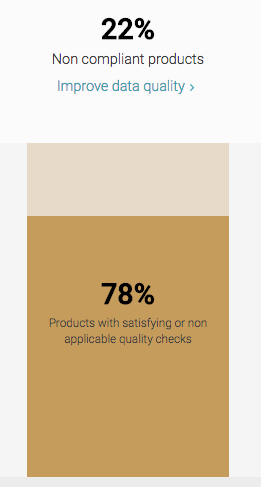
\includegraphics[scale=0.50]{./images/data-quality/data-quality-2.png}
\caption{Example of data-quality measure.}
\end{figure}

Data quality can be evaluated through:
\begin{itemize}
\item completeness: the product page has sufficient details about the product.
	\begin{itemize}
		\item regulatory fields: for instance if your product contains alcohol you must provide the alcohol concentration.
		\item retailer specific fields: some retailer set their own requirements to sell on their platforms
	\end{itemize}
\item accuracy: the provided data is accurate, there is no error.
\end{itemize}

\begin{figure}[H]
\centering
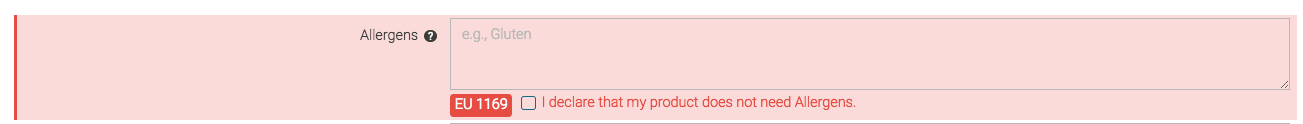
\includegraphics[scale=0.4]{./images/data-quality/data-quality.png}
\caption{Example of a product that doesn't specify required fields.}
\end{figure}

\subsection{Why it matters}

\textbf{Data quality is a major issue to retailers}

\begin{itemize}
\item Regulatory: internet retailers have the obligation to provide some specific informations on the products. If they don't they can be heavily fined. Fields as 
\item Marketing: display detailed information about products to customers. Would you buy products with no description?
\item Search: to correctly index products you need data, for instance how will your customer find strawberry icecream is flavors fields are not well filled. Well indexed products is key to performant search engine on web plateforms.
\item Logistics: weight, size, number of units etc. These fields allow retailers to correctly handle logistics.
\item Competition: the rise of Amazon is a direct threat to all retailers. One of Amazon's advantages is its huge ability to handle data-flows.
\end{itemize}


\subsection{Why is the data of poor quality}

Some of the reasons are:

\begin{itemize}
\item many actors have to communicate: more than 50 thousands of manufacturers have to interact with dozens of retailers. Each manufacturer has to send its data to each retailer sending its products. This represents hundreds of thousands of connections.
\item no fully accepted data-model standard. Even though GDSN standard is dominant, not all companies are compliant with it.
\item actors interested in data-quality (primarly retailers), rely on actors for which it is less crucial (makers)
\item products data identification numbers (EAN) frequently change
\end{itemize}

\subsection{What can we do about data-quality}

Given a product, we want to predict several of its attributes given some basic fields that are nearly always filled.
The predicted fields for now are:
\begin{itemize}
	\item hazard pictograms (inflammable, corrosive etc ...)
	\item labels (organic, made in France, eco-packaging etc...)
	\item kind: category in Alkemics data-model (Processed meat, Cereal, baked product etc...)
	\item allergens (walnut, lactose, sulfite etc ...)
	\item flavors
\end{itemize}

\begin{figure}[H]
\centering
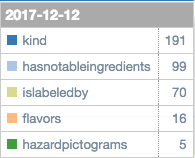
\includegraphics[scale=0.55]{./images/workflow/predicted_fields.png}
\caption{Number of distinct classes per predicted attribute.}
\end{figure}

After these predictions are made, we want to evaluate it against products attributes to warn the manufacturers if we think that some of its data is incomplete or innacurate.

\subsection{What are our constraints}
\begin{itemize}
\item we cannot unilaterally change manufacturers data: they own their data
\item we must garanty a high degree of confidence on suggestions we make, especially at the begining, otherwise manufacturers won't trust and use our suggestions
\item predictions must be made regularly (product data continuously evolve)
\item predictions must adapt to data-model changes
\item our predictive models hade to perform well on datasets of poor data-quality (some fields are nearly never filled)
\item we must be able to monitor closely how well our models perform, and how well perceived are our suggestions 
\end{itemize}


\pagebreak
\section{Suggestion Workflow to improve data-quality}


This part aims at presenting the workflow we use to provide attribute suggestions on product-pages to our users.

During the creation of this workflow, we sticked to some best practices for machine learning engineering, among those listed in a Google paper \cite{RulesMLGoogle} we can cite:
\begin{itemize}
	\item keep the model simple and get the infrastructure right (rule 4)
	\item test the infrastructure independently from the machine learning (rule 5)
	\item starting with an interpretable model makes debugging easier (rule 14)
\end{itemize}

\begin{figure}[H]
\centering
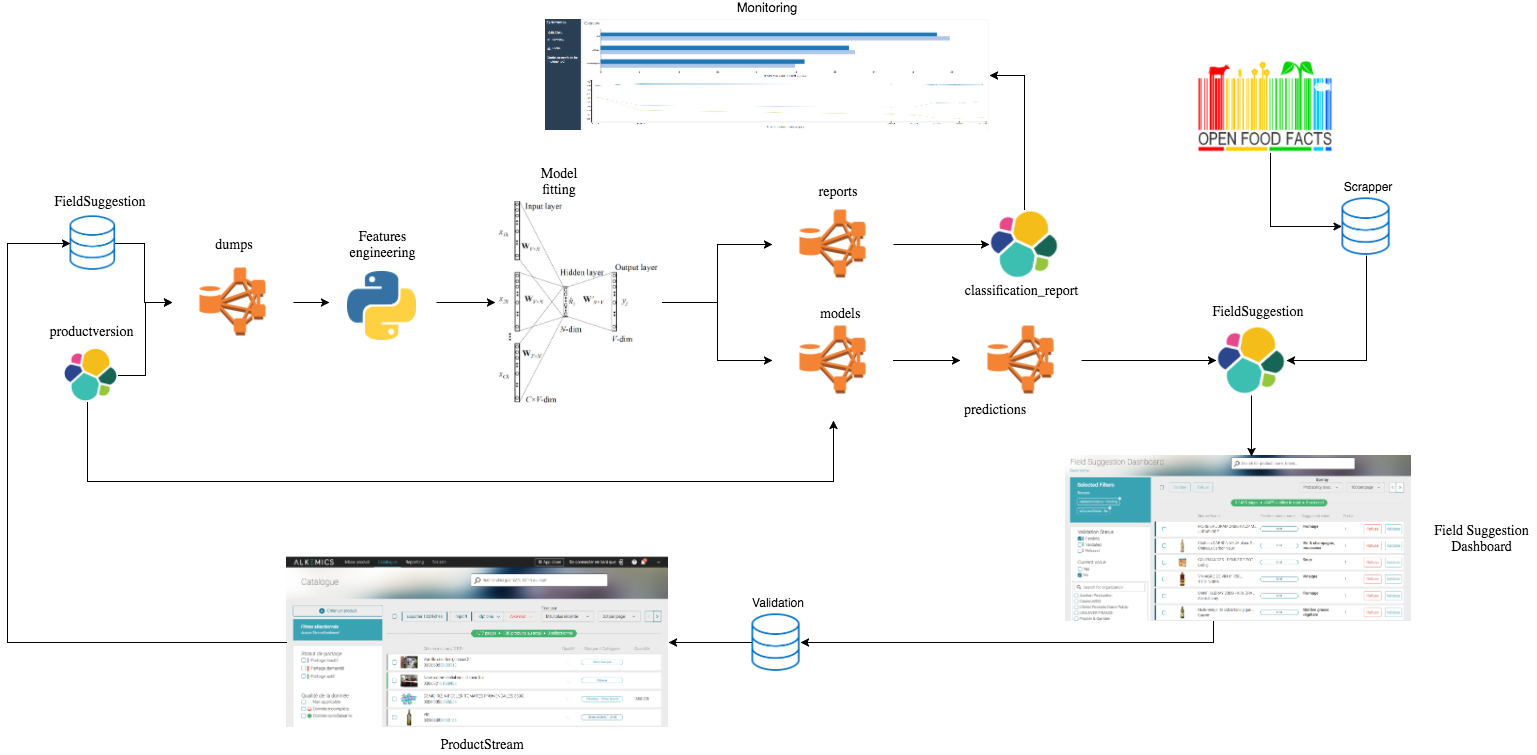
\includegraphics[scale=0.30]{./images/workflow/fieldsuggestion-workflow.png}
\caption{Suggestion workflow overview.}
\end{figure}

\subsubsection{Workflow steps}
\begin{enumerate}
	\item extraction of some attributes (name, description, composition) from products
	\item feature engineering (NLP preprocessing)
	\item training on labeled products (fasttext model) and report
	\item prediction (on all products)
	\item indexation as suggestion
	\begin{itemize}
		\item from machine learning suggestions
		\item from scrapped websites (major one: OpenFoodFacts)
	\end{itemize}
	\item suggestion validation by Alkemics
	\item display of validated suggestions to users in product pages
	\item suggestion acceptation by users
\end{enumerate}


% For product 1198365 / 07622300788063: https://stream.alkemics.com/#/catalog/07622300788063


\subsection{Feature and labels extraction}

In our data-model, a product can consist of more than one hundred of fields, yet only some of them can be sufficient.
The idea is to find a compromise between gathering enough information from products (-> more fields), but on fields with sufficient completion (-> less fields). For now we chose to only use textual data, and let aside pictures (we might use them in the future).

Let's take a cereal bar of brand Grany:
\begin{figure}[H]
\centering

\includegraphics[scale=0.50]{./images/sample/grany_picture.png}
\caption{Product for which we will try to improve data-quality.}
\end{figure}

Here are the extracted attributes that will be processed to provide our features.

\begin{minted}[breaklines, fontsize=\small]{json}
{
    "brand": "Grany",
    "namePublicLong": "Grany Coeur Fondant Gout Chocolat Noisettes 120g",
    "nameLegal": "BARRE CEREALIERE FOURREE AU CHOCOLAT ET A LA NOISETTE.",
    "composition": "Ingrédients: Céréales 31,5% (farine de RIZ 9,1%, farine de BLÉ 5,6%, grains de maïs 4,7%, flocons de BLÉ 4,5%, flocons d'AVOINE 4,5%, flocons d'ORGE 2,5%, farine de BLÉ malté 0,6%), sirop de glucose-fructose, sucre, huile de coprah, LAIT écrémé en poudre, huile de palme, chocolat 5% (sucre, pâte de cacao), pâte de NOISETTES 5%, cacao maigre en poudre, humectant (glycérol), sel, gluten (de BLÉ), dextrose, émulsifiant (lécithine de tournesol), malt d'ORGE, arôme (NOISETTES), ARACHIDE. PEUT CONTENIR SOJA, AUTRES FRUITS À COQUE.",
    "description": "Grany au cœur Chocolat au Lait et aux Noisettes, le plaisir brut des céréales associées au fondant du chocolat au lait !",
    "advices": "",
    "healthAllegations": ""
}
\end{minted}

\subsection{Feature engineering}

Transforming these features in a relevant input format for our models. 
The models we use will be detailed in next chapter. Theses models accept similar input as famous NLP models such skip-gram or c-bow.

This is classic NLP preprocessing.

\begin{enumerate}
	\item concatenated fields as string
	\item normalize text (encoding -> ascii)
	\item tokenize
	\item for each token:
	\begin{itemize}
		\item lower
		\item remove eventual html tags
		\item filter stopwords and punctuation
		\item remove digits
		\item stem (we use NLTK package \cite{NLTK})
	\end{itemize}
	\item concatenate tokens
\end{enumerate}

Our previous object is now a list of preprocessed tokens that take the following form.

\begin{minted}[breaklines, fontsize=\small]{json}
"grany cur chocolat lait noiset plais brut cereal associe fond chocolat lait grany barr cerealier fourre chocolat noiset grany coeur fond gout chocolat noiset ingredient cereal farin riz farin ble grain flocon ble flocon avoin flocon orge farin ble malt sirop glucos fructos sucr huil coprah lait ecrem poudr huil palm chocolat sucr pat cacao pat noiset cacao maigr poudr humect glycerol sel gluten ble dextros emulsifi lecithin tournesol malt orge arom noiset arachid conten soj autr fruit coqu"
\end{minted}

\subsection{Training stage}

Training stage includes:
\begin{enumerate}
	\item labeled-set preprocessing: remove blacklisted labels, filter classes without enough occurences (we want our model to learn only labels we want to display).
	\item split training/testing sets:
	\item fit models on training set, predict on testing set
	\item compute performance and monitoring reports separatly on both train-set and test-set
	\item compute global/local precision curves
	\item save model for further use
	\item index reports for monitoring
\end{enumerate}

Labeled-set preprocessing is not the same in the case we consider multiclass or multilabel classification.
\begin{itemize}
	\item in multiclass case: every sample has one and only one label
	\item in multilabel case: a sample can be considered even though it has no label
\end{itemize}

\subsection{Predict stage}
Predict stage includes: 
\begin{itemize}
	\item extracting all product features (label AND non-labeled)
	\item compute prediction scores
	\item enrich prediction with recall/precision estimations based on prediction score and local precision/recall curves computed during training-stage
	\item save all predictions with scores > 0.05
\end{itemize}

\subsection{Machine learning suggestion indexation with scrapped information}

Suggestions from machine learning, are merged with suggestions issued from web-scrapping.
Those suggestions are indexed together to provide a global score (number of concordant sources) to suggestions.

Here is an example of a suggestion document that will be indexed in ElasticSearch. Its structure will allow us to perform complex queries and provide a validation dashboard with many functionalities.
\begin{minted}[breaklines, fontsize=\small]{json}
{
    "_type": "fieldsuggestion",
    "extended_attributes": {
        "precision_group": 0.91489,
        "features": "grany cur chocolat lait noiset plais brut cereal...",
        "probability": 0.87393,
        "recall_group": 0.55128
    },
    "field": {
        "status": 0,
        "fieldmetadata_name": "hasnotableingredients",
        "fieldmetadata_id": 107,
        "is_current_value": 0,
        "field_id": 59,
        "field_name": "arachide"
    },
    "id": "1198365_107_59",
    "metadata": {
        "global_score": 4,
        "product_id": 142292,
        "media": "https://smedia.alkemics.com/product/142292/...",
        "brand": "Grany",
        "contentowner": {
            "id": 356,
            "name": "Mondelez International"
        },
        "sources": [
            "openfoodfacts",
            "ml"
        ],
        "gtin": "07622300788063",
        "productversion_id": 1198365,
        "name": "Grany Coeur Fondant Gout Chocolat Noisettes 120g"
    }
}
\end{minted}


\subsection{Validation (or refusal) from Alkemics}
Since we must reach a high degree of confidence in our predictions, and since we do not yet have history about how well we perform, each suggestion is manually validated. 


For all predictions that are not values already stored in products' data (if the prediction match an already existing product data, everything's fine and we don't need to change its value), we will validate or refuse the suggestion.

A part of this task is semi-automated: for instance, suggestions issued from both scrapping and machine learning, with an estimated precision of 90\% are batch validated.

\begin{figure}[H]
\centering
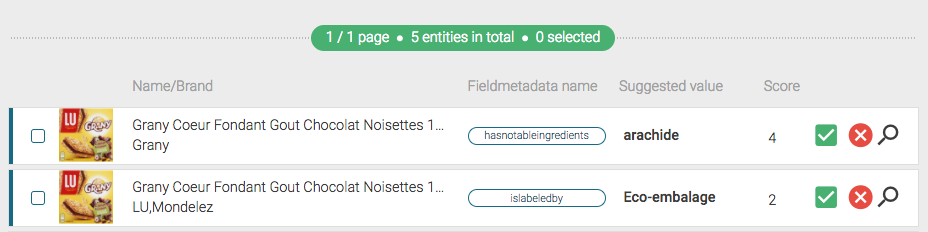
\includegraphics[scale=0.40]{./images/workflow/validation-suggestion.png}
\caption{Suggestion validation by Alkemics.}
\end{figure}


\subsection{Suggestion display to users in product pages, and acceptation (or dismissal) from manufacturer}

Now that the suggestion is validated, we notify the manufacturer in charge of this product, and include a control in his product page allowing him to easily accept of dismiss the suggestion.

\begin{figure}[H]
\centering
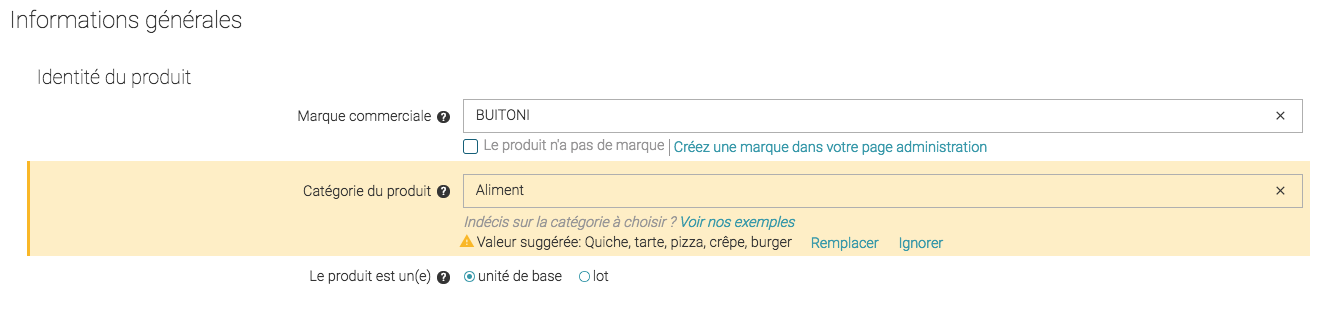
\includegraphics[scale=0.35]{./images/workflow/stream-suggestion-3.png}
\caption{Suggestion acceptation by user.}
\end{figure}

In case of acceptation, the product's data is changed in Alkemics product database. Else, in case of dismissal, we store the fact that the suggestion is 'wrong' so we don't notify the manufacturer if we repredict the same value the day after.


\pagebreak
\section{Regular maintenance and improvement tasks}

Once the workflow is deployed there are several day-to-day tasks to perform. This include monitoring the workflow to detect eventual anomalies, validating suggestions so that they are sent to users, and manually bootstrapping some classes for which our models don't perform well.

\subsection{Monitoring}

Given the complexity of the workflow, and quality expected by clients, we have to closely monitor some metrics:
\begin{itemize}
	\item did the workflow worked, if not where did it fail
	\item is there an evolution of classes distribution
	\item how our scores behave at training stage
	\item whether our predictions get rejected at validation stage
	\item do our validated suggestion get dismissed by user at acceptation stage
\end{itemize}

\subsubsection{Check workflow completion}
Our workflow consists of lots of interdependent tasks. Some of them have to be completed in a precise order. Some can be parallelized, some not. To ensure that our workflow runs as expected we use a workflow management tool: Luigi.

By defining each task dependencies (a task can depend on multiple other tasks), Luigi will draw an acyclic directed dependency graph.

Luigi library comes with a useful web interface, showing wich tasks are pending/runing/completed or have failed:
\begin{figure}[H]
\centering
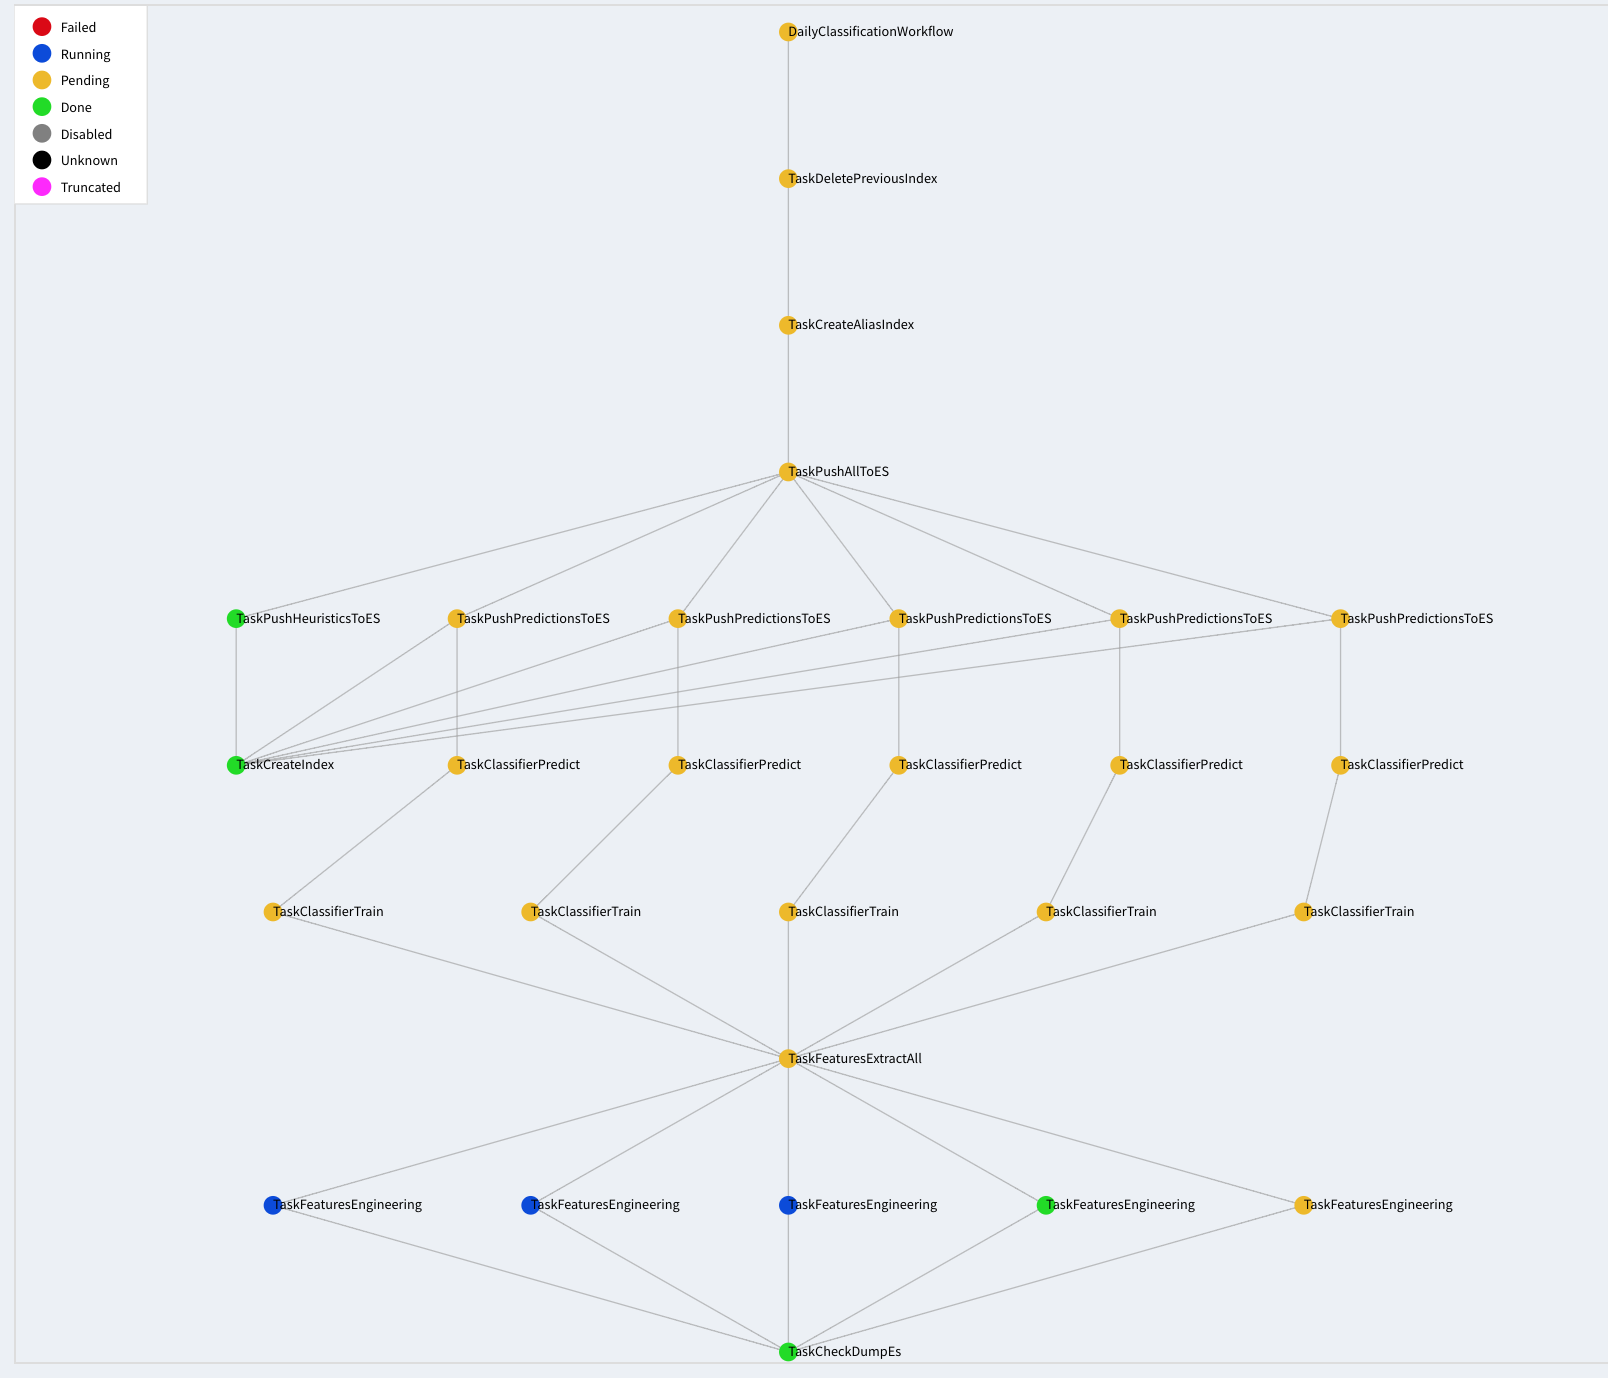
\includegraphics[scale=0.50]{./images/monitoring/luigi-graph-3.png}
\caption{Classification workflow dependency graph.}
\end{figure}

\subsubsection{See and understand scores evolution}
Knowing how our models perform is crucial to know how confident we can be into our models.

To do so I built a monitoring interface drawing the scores evolution for different fields we try to enrich.
\begin{figure}[H]
\centering
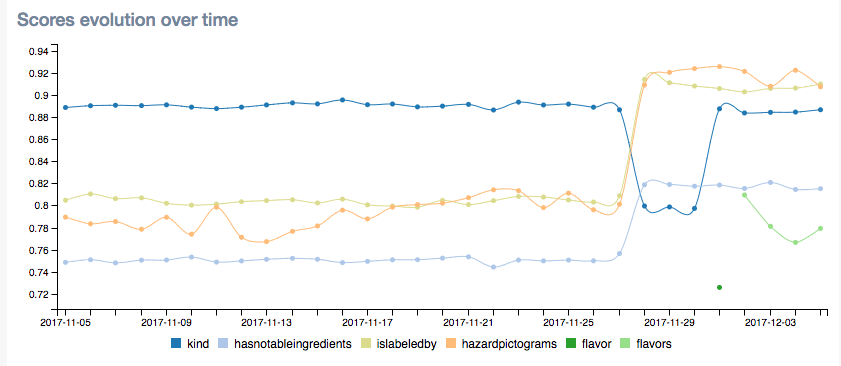
\includegraphics[scale=0.50]{./images/monitoring/global-scores-evolution-2.png}
\caption{Classification micro-average global scores evolution.}
\end{figure}

Among the different reasons why our models scores can evolve, one is the change of classes distribution, so some graphs can help check if something is wrong: in this case, the following graph helped us find why a field predictions dropped: some wrongly labeled data was introduced.

\begin{figure}[H]
\centering
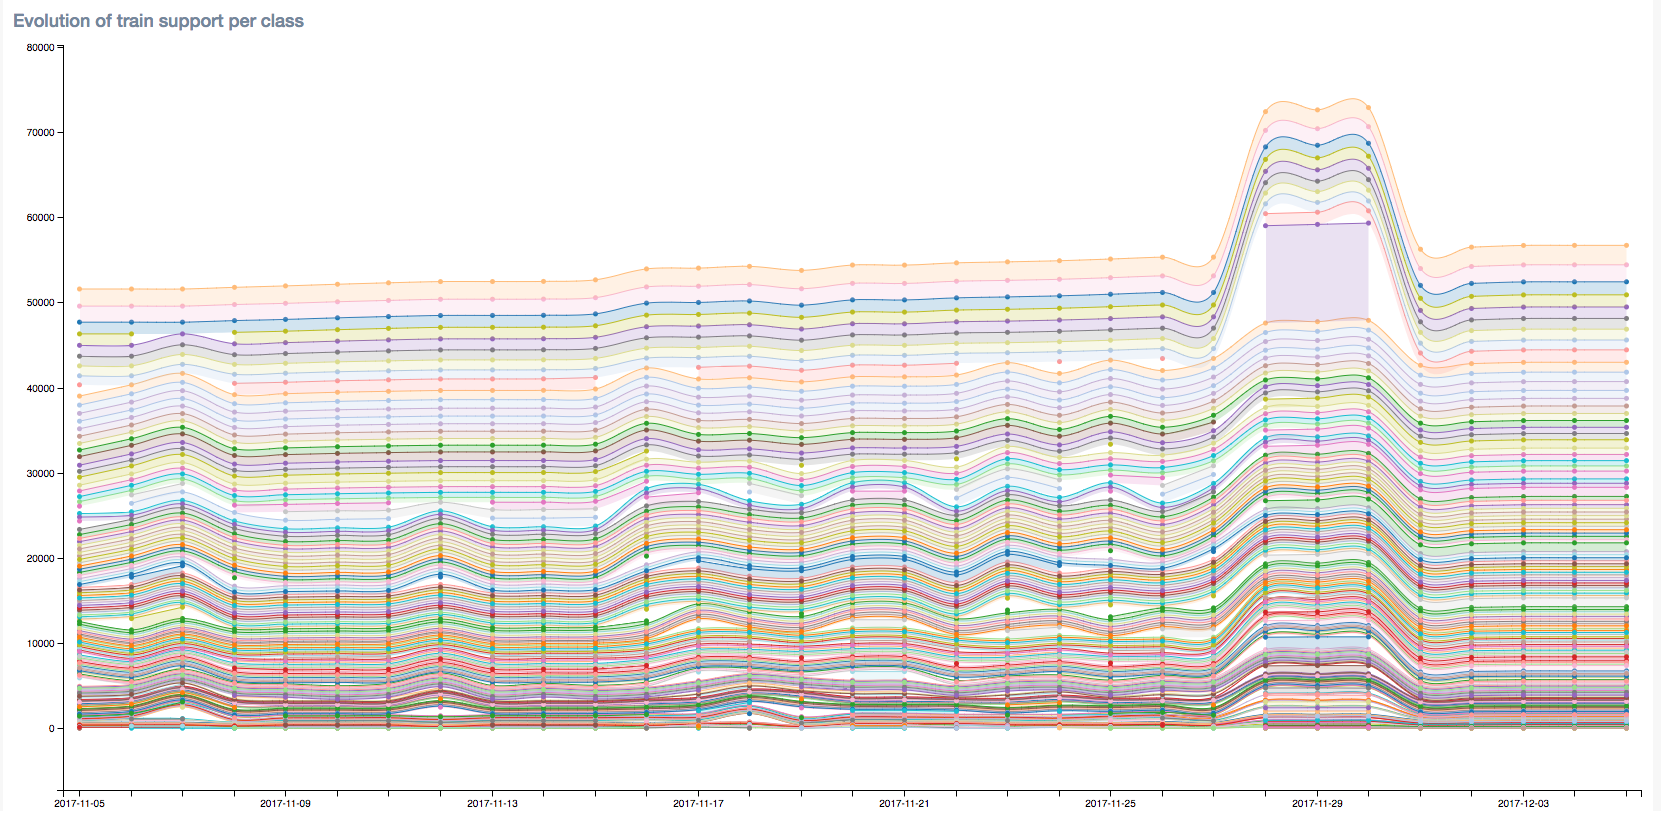
\includegraphics[scale=0.30]{./images/monitoring/local-classes-evolution.png}
\caption{Local classes distribution evolution. We can detect the creation of an invalid class that led to dropping scores.}
\end{figure}


\subsubsection{Check validation / Acceptation rates}

In machine learning, the more frequent way to estimate a model performance is to predict on a test-set and compare predictions to true labels of the test-set.

In our case, we can also check the validation/refusal ratio at validation stage:

\begin{figure}[H]
\centering
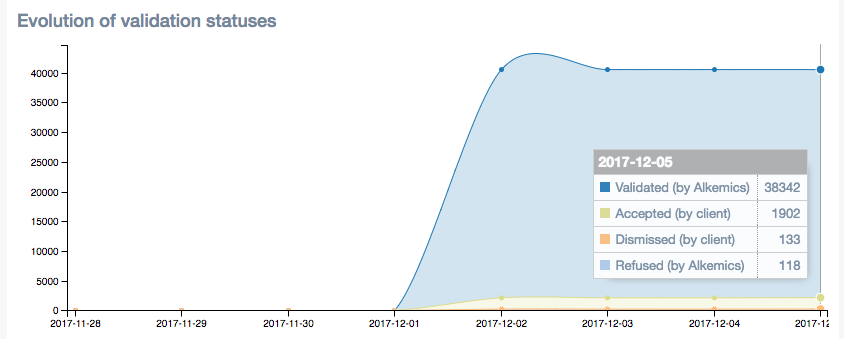
\includegraphics[scale=0.5]{./images/monitoring/validation-acceptation-monitoring.png}
\caption{Validation/Acceptation rates.}
\end{figure}

\subsubsection{Evaluate business impact}

Number of views, and acceptation rates.

\subsection{Deliver validated suggestions}

By a mix of automation and manual validation.
A big effort has been made to build an internal suggestion validation dashboard. 

\begin{figure}[H]
\centering
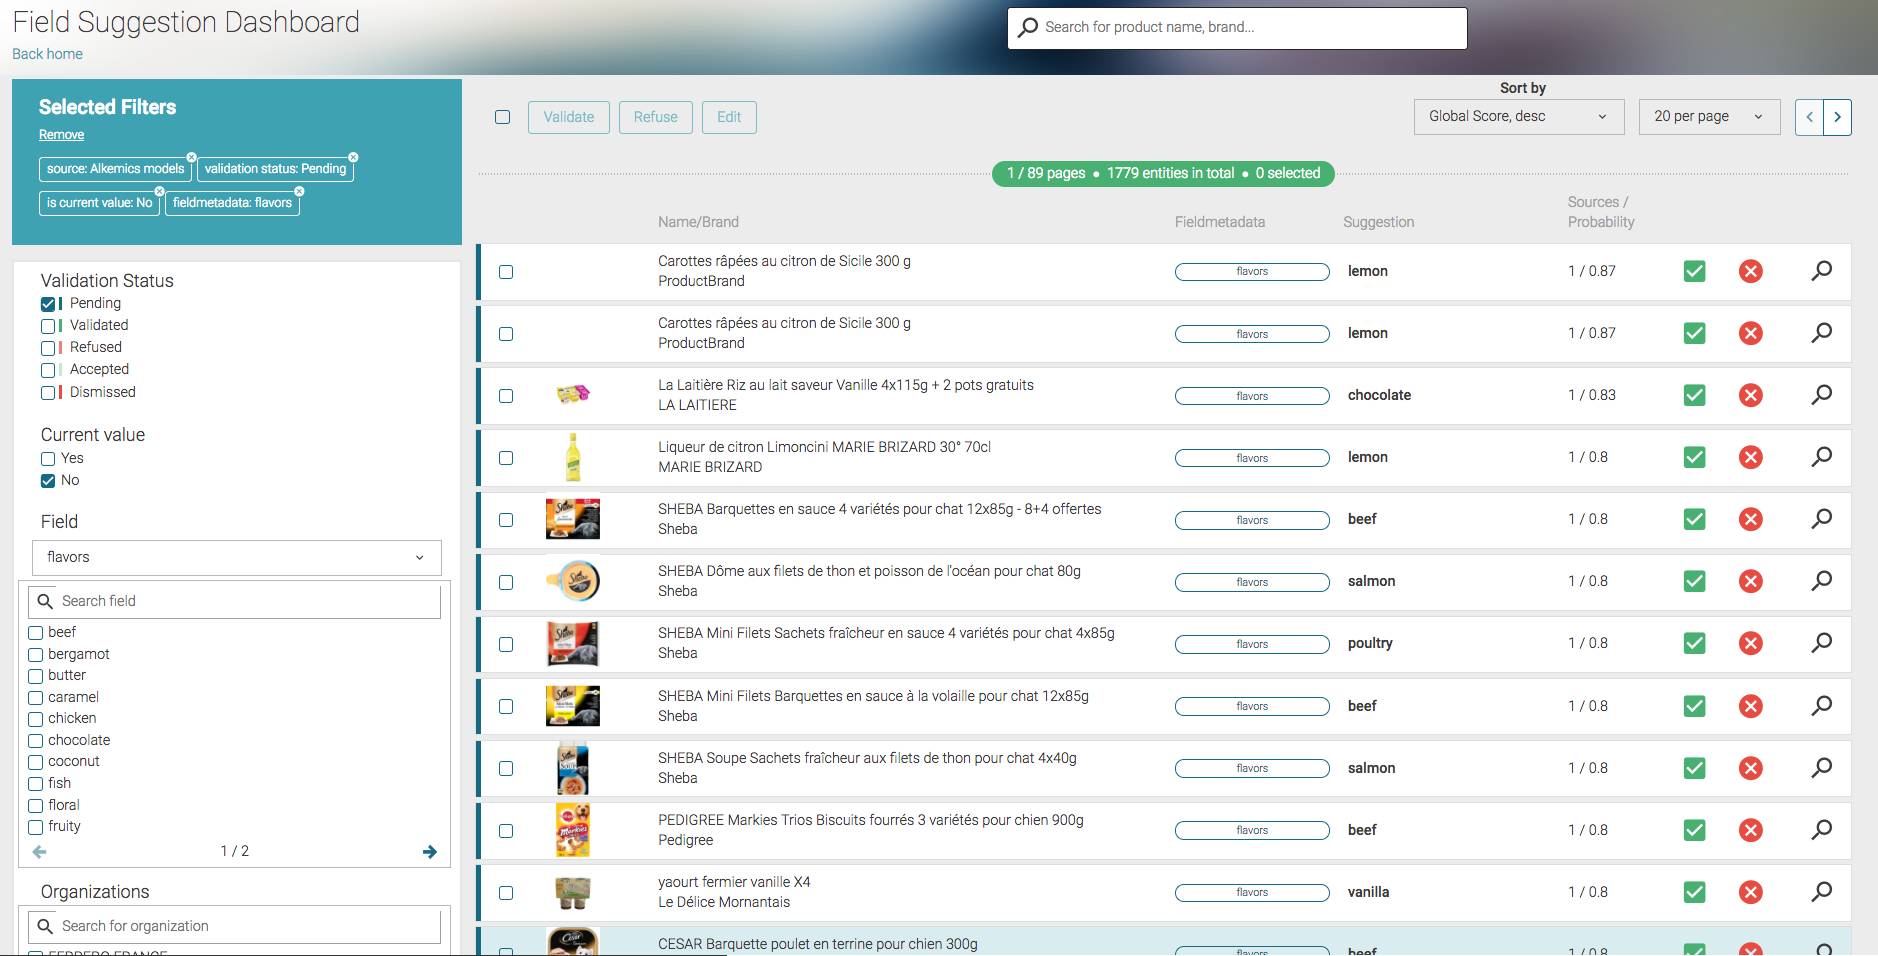
\includegraphics[scale=0.54]{./images/data-quality/validation-dashboard.png}
\caption{Validation dashboard.}
\end{figure}

This dashboard allows us to easily filter suggestions based on:
\begin{multicols}{2}
\begin{itemize} 
	\item validation/acceptation status
	\item is prediction a the current value
	\item field (flavors, kind...)
	\item classes (gluten, lactose...)
	\item organizations
	\item source 
	\item score 
\end{itemize}
\end{multicols}

For instance it is thus possible to easily select suggestions whose validation status is pending, and that do not match current values in database. We can then sort these suggestions by number of different sources and filter those with sufficient precision estimation, and validate suggestions in batches.


\subsection{Tune fasttext hyperparameters}

Each predicted field data-set has different charateristics:
\begin{itemize}
	\item number of different classes (5 to 175)
	\item classes disparity: some fields have very distinct classes, whereas some others have very related classes.
	\item label density (for multilabel): do your products have on average 1 label or 5 different labels
\end{itemize}

Then, each of these tasks might require different model hyper-parameters (those parameters will be detailed in the next chapter).
That's why we build a service on a dedicated machine whose goal is to find the best parameters.

\subsection{Bootstrap new classes/fields}

Everyday at Alkemics, clients use our plateform, and the data changes. Thus, unlike in kaggle competition, our datasets evolves.
For instance, some new ingredients might appear, and at the beginning their low number of occurence might prevent the model to perform well.

\begin{figure}[H]
\centering
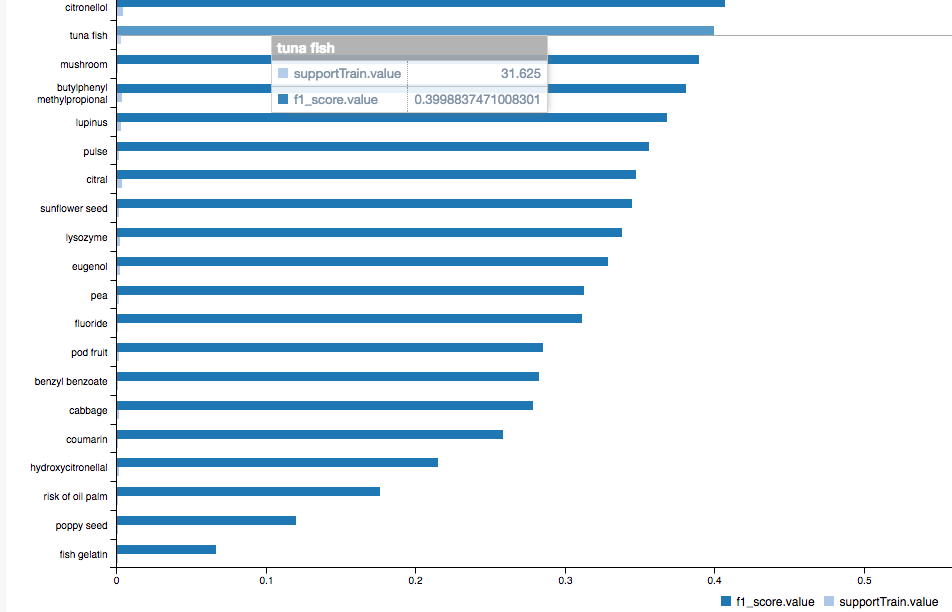
\includegraphics[scale=0.5]{./images/data-quality/islabeledby_support_score.png}
\caption{Selection of classes with lowest scores. Tuna fish performs badly, because of the low train support.}
\end{figure}

In that case we will use our validation dashboard. We would make a textual search to validate some related suggestions, or even create manually some suggestions. Sometimes, even some dozens of occurences are enough to bootstrap a new class and launch a virtuous circle for the model.

This process will be covered in the next chapter, here \ref{fig:textualvalidation}.


